\documentclass{beamer}
% \usetheme{Madrid}
% \usetheme{Madrid}
\usetheme{Frankfurt}
\usepackage{amsfonts}  % for \mathbb
\usepackage{amsmath}  % for \mathbb
\usepackage{amssymb}  % for \mathbb
\usepackage{graphicx}  % for includegraphics
\usepackage{animate}  % for gifs
\newcommand{\Matrix}[1]{\boldsymbol{#1}}
\newcommand{\Vector}[1]{\boldsymbol{#1}}
\title{Numerical Continuation for Flutter}
\author{Ed Meyer	\\ \texttt{flapsconsulting@gmail.com}}
\date{Dec. 10 2024}
\begin{document}

\begin{frame}
	\titlepage
\end{frame}

\begin{frame}
	\frametitle{3 phases of flutter prediction}
	\begin{itemize}
		\item Analysis
			\begin{itemize}
				\item starts early in the design of a new airplane
				\item continues through flight test and FAA certification
			\end{itemize}
		\item Wind tunnel tests: not always
		\item Flight test
			\begin{itemize}
				\item fly at various speeds, altitudes, and maneuvers
				\item usually accompanied by a chase plane to look for flutter
			\end{itemize}
	\end{itemize}

	\vspace{5mm}
	``Everyone believes the flight test except the person who ran the test,
  no one believes the analysis except the person who did the analysis''
\end{frame}

\begin{frame}
	\frametitle{2 types of flutter}
	\begin{itemize}
	\item destructive flutter
		\begin{itemize}
			\item oscillations grow until something breaks
			\item usually catastrophic
		\end{itemize}
	\vspace{5mm}
	\item limit-cycle oscillations (LCO)
		\begin{itemize}
%			\item displacement amplitudes limited by some mechanism like stiffness that
%				varies with displacement
 			\item displacement amplitudes limited by some force that varies with
				displacement, e.g. stiffness or aerodynamics
			\item not immediately destructive, but might fatigue
			\item analysis must take nonlinearities into account to predict LCO
		\end{itemize}
	\end{itemize}
\end{frame}

\begin{frame}
	\frametitle{Destructive flutter in flight test}
	Flight testing a 707 modified for the Navy encountered tail flutter. The pilot
	managed to land with the top half of the tail broken off

 	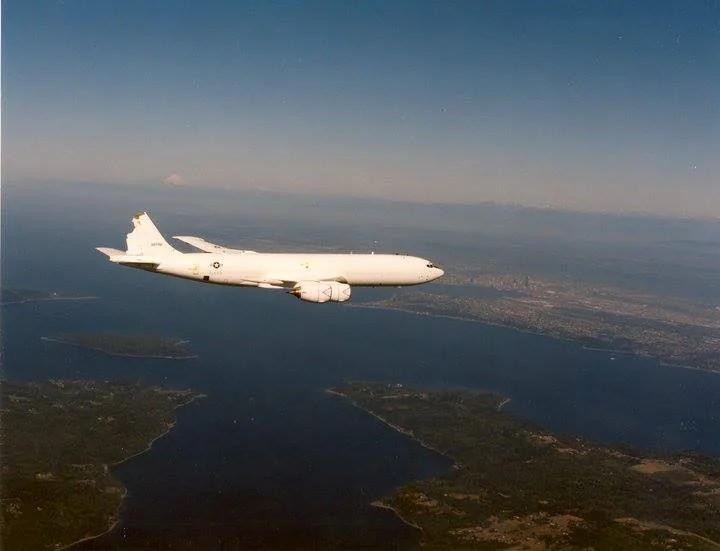
\includegraphics[height=7cm,width=9cm]{e6.jpg}
\end{frame}

\begin{frame}
	\frametitle{Destructive whirl flutter}
	Lockheed L-188 Electra crashed twice due to whirl flutter

	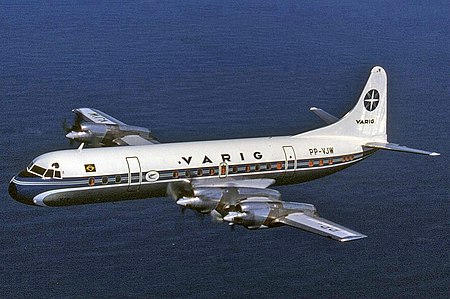
\includegraphics[height=7cm,width=9cm]{lockheed-L188.jpg}
\end{frame}

\begin{frame}
	\frametitle{Whirl flutter}
	Propeller driven aircraft are subject to an instability caused
	by propeller aerodynamics and gyroscopics

	\animategraphics[width=10cm,autoplay,loop]{5}{whirl}{2}{40}
\end{frame}

\begin{frame}
	\frametitle{LCO in the wind tunnel}
%	An early version of the Lockheed L-10 Amelia Earhart died in
%	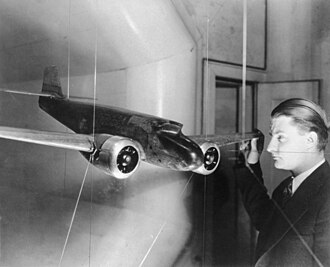
\includegraphics[height=7cm,width=9cm]{Kelly-Johnson_Electra.jpg}
%	\includegraphics[height=7cm,width=9cm]{windtunnelLCO.gif}
% 	\animategraphics[width=10cm,autoplay,loop,convert]{5}{windtunnelLCO.gif}{1}{29}
 	\animategraphics[width=10cm,autoplay,loop]{5}{wtun-}{1}{4}
%	\animategraphics[width=10cm,autoplay,loop]{5}{wtLCO-}{1}{5}
\end{frame}

\begin{frame}
	\frametitle{LCO in flight test}
	An early version of the 737 had elevator buzz which might eventually have fatigued something
%	\animategraphics[width=10cm,autoplay,loop]{5}{elevator}{5}{40}
 	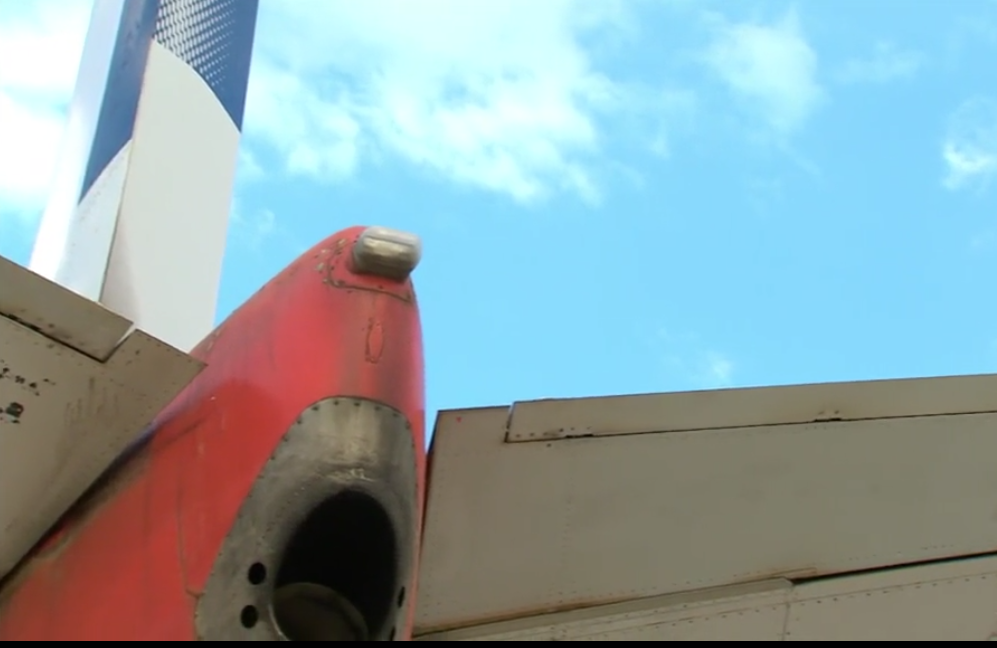
\includegraphics[height=7cm,width=9cm]{tab.png}

\end{frame}

\begin{frame}
	\frametitle{The flutter equation: $\Vector{Dy} = \Vector{0}$}
	\begin{itemize}
		\item The \emph{linear} flutter equation is independent of the amplitude
			of oscillation...
		\item but it is a \emph{nonlinear} function of parameters
		   such as velocity, frequency, and stability factor ($\sigma$)
			\begin{itemize}
				\item homogeneous in the amplitude of oscillation ($\Vector{y}$)
				\item gives no indication as to whether an instability is destructive flutter
					or an LCO
			\end{itemize}
%		\item The nonlinear flutter equation depends on the amplitude of oscillation
		\item If the flutter equation is dependent on the amplitude of oscillation is is
			a \emph{nonlinear flutter equation} and it
			\begin{itemize}
				\item is more realistic
				\item is harder to solve
				\item determines whether a solution is LCO or destructive flutter
			\end{itemize}
	\end{itemize}
\end{frame}

\begin{frame}
	\frametitle{Vibration}
	The vibration problem,
	\begin{equation}\label{eqn:vibe}
%		\left[ -\omega^2 \Matrix{M} + \Matrix{K}\right]\Vector{y} = \Vector{0} \nonumber
		\Matrix{K}\Vector{y} = \omega^2 \Matrix{M}\Vector{y} \nonumber
	\end{equation}
	where $\omega$ is the frequency, is a generalized, symmetric eigenvalue problem
	usually written as
	\begin{equation}
		\Matrix{A}\Vector{x} = \lambda \Matrix{B}\Vector{x}
	\end{equation}

	\vspace{5mm}
	which has real eigenvalues and eigenvectors provided the eigenvalues of $\Matrix{M}$ are $> 0$
%	ICBS if $\Matrix{M}$ and $\Matrix{K}$ are symmetric $-\omega^2$ is real so if
%	frequency $\omega$ is $\ge 0$ provided $\omega^2 \ge 0$
%	\begin{description}
%		\item[$-\omega^2 \le 0$] the frequency $\omega = \sqrt{\omega^2}$
%		\item[$-\omega^2 > 0$] the structure is unstable
%	\end{description}
\end{frame}

\begin{frame}
	\frametitle{Add structural damping}
	\begin{equation}\label{eqn:sdamp}
		\left[ s^2 \Matrix{M} + (1+id)\Matrix{K}\right]\Vector{y} = \Vector{0} \nonumber
	\end{equation}

	\vspace{5mm}
	Now the eigenvalue $s = \sigma + i\omega$ is complex and $\sigma$ determines the stability of
	the structure:
	\begin{description}
		\item[$\sigma \le 0$] oscillations decay, structure is stable
		\item[$\sigma > 0$] oscillations grow, structure is unstable
	\end{description}
	where $i = \sqrt{-1}$ and $d$ is the structural damping coefficient.
\end{frame}

\begin{frame}
	\frametitle{Add aerodynamics}
	\begin{equation}\label{eqn:sdamp}
		\left[ s^2 \Matrix{M} + (1+id)\Matrix{K} -q\Matrix{A}\right]\Vector{y} = \Vector{0} \nonumber
	\end{equation}

	\vspace{5mm}
%	where $\bar{s} = \frac{sb}{V} = \frac{\sigma b}{V} + i\frac{\omega b}{V}$ and $M$ is the Mach number,
	where $q = \rho V^2/2$ is the dynamic pressure.

	\vspace{5mm}
	\begin{itemize}
		\item {\bf challenging} to solve as an eigenvalue problem
		\item still widely used solution technique
	\end{itemize}
\end{frame}

\begin{frame}
	\frametitle{Add gyroscopics, viscous damping, control system, parameters, nonlinearities}
	\begin{equation}\label{eqn:flut}
		\left[ s^2 \Matrix{M} + s \Omega\Matrix{G} + s \Matrix{V} +
		 (1 + id) \Matrix{K}(\Vector{y}) - q \Matrix{A} (\bar{s},M) + \Matrix{T} \right]
		  \Vector{y} = \Matrix{D}\Vector{y} =
		  \Vector{0} \nonumber
		\end{equation}

	\begin{description}
		\item[$\Matrix{G}$, $\Matrix{V}$] are gyroscopic and viscous damping matrices,
		\item[$\Matrix{T}$] a user-defined matrix (e.g. control-system equations),
		\item[$\Matrix{D}$] the complex dynamic matrix.
	\end{description}

	\vspace{5mm}
	impossible to solve as an eigenvalue problem
\end{frame}

\begin{frame}
	\frametitle{Solve as a system of nonlinear equations}
	A system of $n$ nonlinear equations in $n$ unknowns,
	\begin{equation}
		\Vector{f}(\Vector{x}) = \Vector{0}	\nonumber
	\end{equation}

	\vspace{5mm}
	is often solved with Newton's method:
	\begin{equation}
		\Vector{x}^{j+1} = \Vector{x}^{j} - \Matrix{J}^{-1}\Vector{f}(\Vector{x}^{j})	\nonumber
	\end{equation}
	\vspace{5mm}
	the $n$ complex flutter equations $\Matrix{D}\Vector{y} = \Vector{0}$ are equivalent to a system of
	$2n$ real nonlinear equations
\end{frame}

\begin{frame}
	\frametitle{Advantages}
	\begin{itemize}
		\item Solve a wide variety of flutter problems
		\item nonlinear flutter is treated the same as linear flutter
		\item Can choose which modes to track
		\item Modes can be tracked in parallel
		\item not necessary to approximate aerodynamics to reduced frequency
	\end{itemize}
\end{frame}

\begin{frame}
	\frametitle{Comparison of 2 modes using 4 different interpolations}
		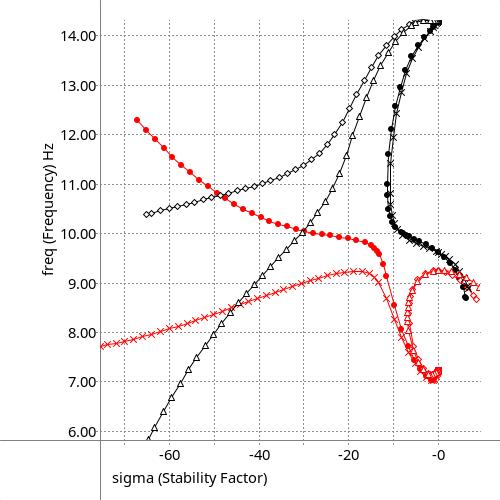
\includegraphics[height=7cm,width=9cm]{dlm.jpg}

			$\bar{\omega}$, $\bar{\omega}$-$\bar{\sigma}$,
			$\bar{\omega}$-$M$, $\bar{\omega}$-$\bar{\sigma}$-$M$
%		\begin{itemize}
%			\item $\bar{\omega}$
%			\item $\bar{\omega}$-$\bar{\sigma}$
%			\item $\bar{\omega}$-$M$
%			\item $\bar{\omega}$-$\bar{\sigma}$-$M$
%		\end{itemize}

\end{frame}

\begin{frame}
	\frametitle{Disadvantages}
	\begin{itemize}
		\item Possible to miss an important mode by limiting the
		number of modes tracked
		\item More expensive than eigenvalue techniques?
	\end{itemize}
\end{frame}

\begin{frame}
	\frametitle{Numerical continuation}
	\begin{itemize}
		\item A general numerical technique for tracing solutions of parameterized nonlinear equations
		\item $n$ equations in $n+1$ unknowns $\Vector{f}(\Vector{x}) = \Vector{0}$
		\item similar to predictor-corrector differential equation solvers
		\begin{itemize}
			\item predictor: $\Vector{x}_{j+1} = \Vector{x}_j + \Delta \tau \Vector{t}$
			\item corrector: Newton's method
		\end{itemize}
	\end{itemize}
\end{frame}

\begin{frame}
	\frametitle{Application: basic flutter}
	Start at zero velocity, compute $s = \sigma + i\omega$, search for
	neutral stability: $\sigma = 0$
	\animategraphics[width=10cm,autoplay,loop]{5}{nacpv}{5}{40}
\end{frame}

\begin{frame}
	\frametitle{Application: parameter variations}
	Starting from a point in the basic solution (usually where $\sigma=0$)
	trace a curve varying some parameter, holding $\sigma$ constant.
		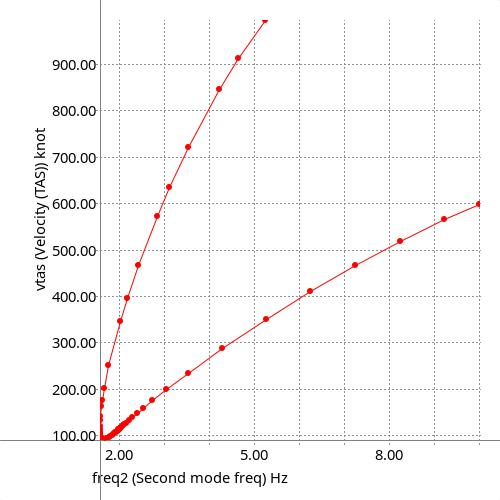
\includegraphics[height=5cm,width=7cm]{freq2.jpg}
\end{frame}

\begin{frame}
	\frametitle{Application: optimization}
	Continuation can be used to optimize a parameter with respect to
	2 or more other parameters: at each step the tangent is computed as
	the direction where the optimization parameter has the greatest increase
\end{frame}

\begin{frame}
	\frametitle{Application: contours}
	the optimization curve is a starting point for all the contours
		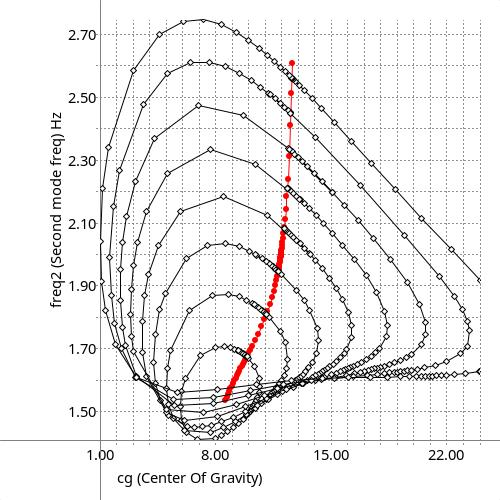
\includegraphics[height=7cm,width=9cm]{contour.jpg}
\end{frame}

\begin{frame}
	\frametitle{Application: nonlinearities}
	Treating the flutter equations as nonlinear equation means it is
	easy to add nonlinearities. Some common nonlinearities treated at
	Boeing are freeplay in control surfaces and nonlinear stiffnesses
\end{frame}

% \begin{frame}
% 	\frametitle{Application: rudder LCO}
% 	freeplay in control surfaces can lead to a type of instability
% 	called Limit Cycle Oscillation or LCO

% 	\vspace{5mm}
% 	\animategraphics[width=7cm,autoplay,loop]{5}{rudder}{2}{40}
% \end{frame}

\begin{frame}
	\frametitle{Application: latent LCO}
		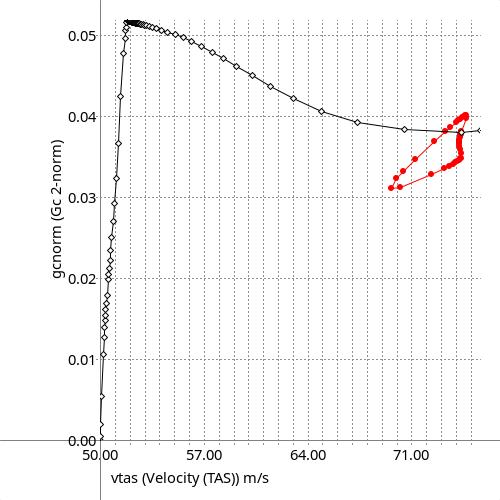
\includegraphics[height=7cm,width=9cm]{latent.jpg}
\end{frame}

\begin{frame}
	\frametitle{Application: control systems}
	The $\Matrix{T}$ matrix is created with a function
	written by the user in C++

	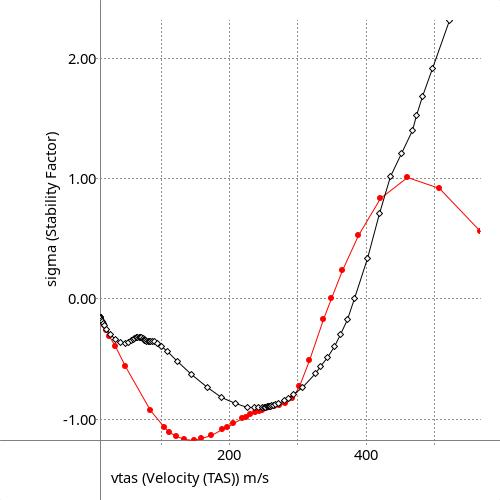
\includegraphics[height=7cm,width=9cm]{controls.jpg}
\end{frame}

\end{document}
